\section{Auswertung}
\label{sec:Auswertung}

\subsection{Aufnahme der Zählrohr-Charakteristik}

\begin{table}[H]
  \centering
  \begin{tabular}{c|c|c|c}
    \hline
    $U$ / V & N / 10\,s & N / $\frac{1}{\text{s}}$ & $\frac{\sqrt{N}}{N}$ \\
    \hline
    350 & 5437 & $\num{544 +- 7}$ & 0.01 \\
    375 & 5384 & $\num{538 +- 7}$ & 0.01 \\
    400 & 5368 & $\num{537 +- 7}$ & 0.01 \\
    450 & 5405 & $\num{541 +- 7}$ & 0.01 \\
    500 & 5447 & $\num{545 +- 7}$ & 0.01 \\
    550 & 5552 & $\num{555 +- 7}$ & 0.01 \\
    600 & 5485 & $\num{549 +- 7}$ & 0.01 \\
    625 & 5598 & $\num{560 +- 7}$ & 0.01 \\
    650 & 5745 & $\num{575 +- 8}$ & 0.01 \\
  \end{tabular}
  \caption{}
  \label{tab:}
\end{table}

\begin{figure}[H]
  \centering
  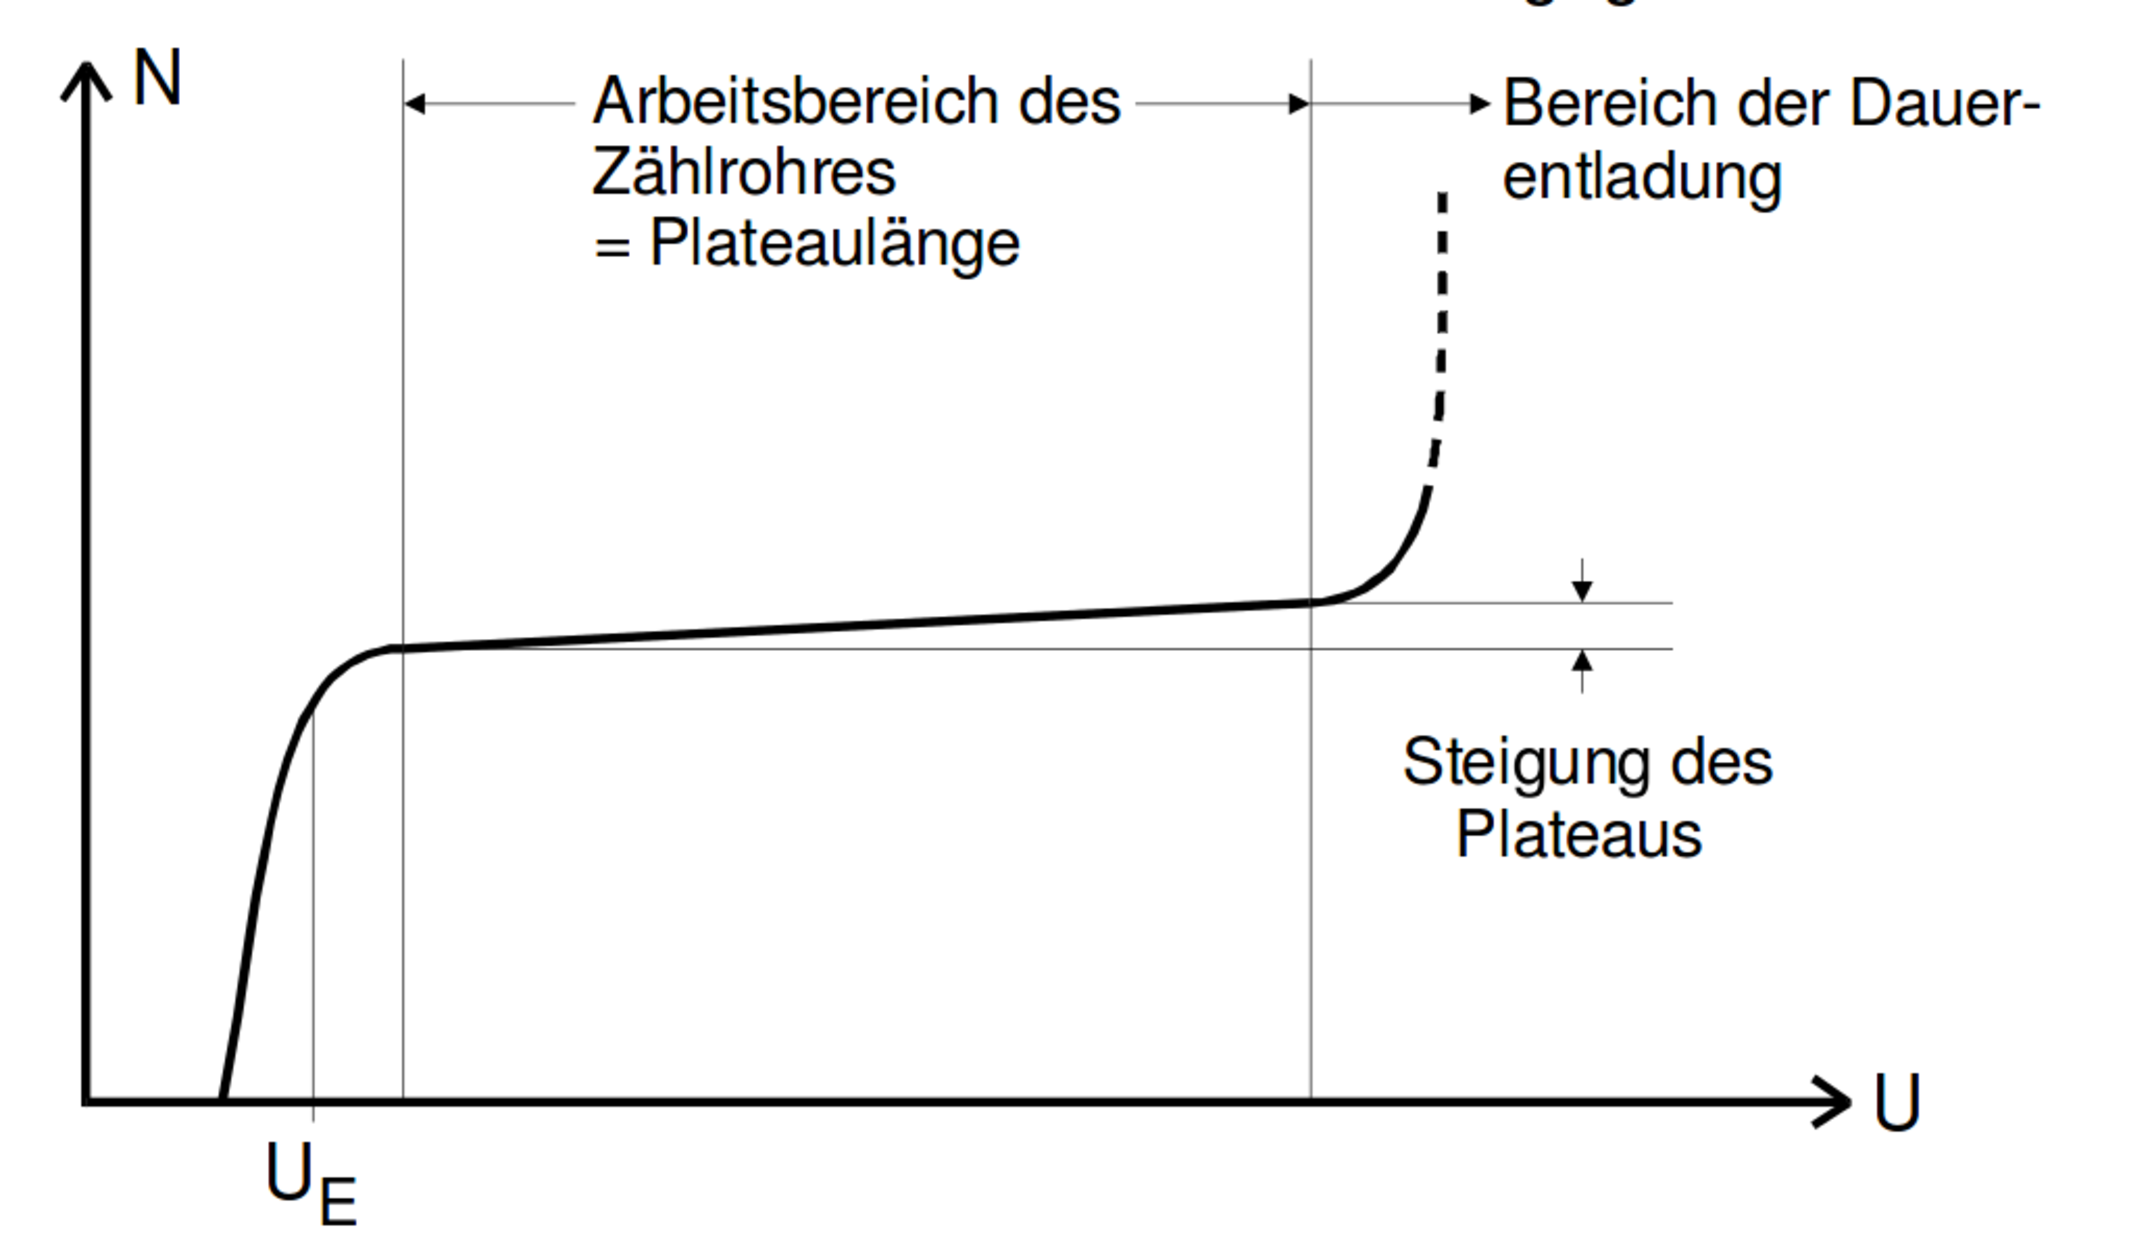
\includegraphics[height=5cm]{build/Plateau.pdf}
  \caption{Charakteristik des Zählrohres.}
  \label{fig:Plateau}
\end{figure}
